\documentclass[12pt,a4paper]{article}

\usepackage{fontspec}
\setmainfont{Times New Roman}

\usepackage[margin=2.5cm]{geometry}
\usepackage{amsmath}
\usepackage{graphicx}
\usepackage{booktabs}
\usepackage{caption}
\usepackage{longtable}
\usepackage{hyperref}
\usepackage{xcolor}
\usepackage{float}

\renewcommand{\figurename}{Hình}
\renewcommand{\tablename}{Bảng}
\renewcommand{\contentsname}{Mục lục}

\hypersetup{
  colorlinks=true,
  linkcolor=black,
  urlcolor=blue,
  citecolor=black,
}

\graphicspath{{../E1/results/}}

\title{\textbf{Báo cáo bài tập E1--E3}\\[0.3em]
\large Học sâu và ứng dụng trong thị giác máy tính\\
Mã môn học: CO5085, Học kỳ 261 (2026--2027)}

\author{
Nguyễn Xuân Trường (2570526) \\
Trần Lê Hoàng Long (2570443)
}
\date{Cập nhật lần cuối: 01/11/2026}

\begin{document}

\maketitle

\vspace{1cm}
\begin{center}
\begin{tabular}{ll}
\textbf{Giảng viên hướng dẫn:} & Lê Thành Sách, Nguyễn Quốc Minh \\
\textbf{Repository:} & \url{https://github.com/truong1501/SDH_HK261_CO5085} \\
\end{tabular}
\end{center}

\clearpage
\tableofcontents
\clearpage

\section{Dữ liệu và protocol dùng chung cho E1--E3}

\subsection{Tập dữ liệu: Fashion-MNIST}

Cả ba bài E1, E2, E3 dùng chung một tập ảnh nhỏ là Fashion-MNIST: ảnh xám
$28 \times 28$, 10 lớp trang phục (T-shirt/top, Trouser, Pullover, Dress, Coat,
Sandal, Shirt, Sneaker, Bag, Ankle boot), mỗi lớp cân bằng số lượng ảnh.

Nhóm chọn Fashion-MNIST thay vì MNIST vì MNIST quá dễ, cả ba kiến trúc
softmax/MLP/CNN thường đạt accuracy rất cao và gần nhau (trên 97\%), khó thấy
rõ chênh lệch về khả năng biểu diễn giữa các kiến trúc cũng như khó phân tích
trường hợp sai. Fashion-MNIST giữ nguyên kích thước và số lớp như MNIST nên
không làm tăng chi phí tính toán, nhưng khó hơn đáng kể (nhiều lớp trang phục
có hình dạng tương tự nhau khi nhìn ở độ phân giải thấp), nên chênh lệch giữa
ba mô hình thể hiện rõ và có nhiều trường hợp sai đáng để phân tích. Nhóm
không chọn CIFAR-10 vì ảnh màu 3 kênh sẽ làm thời gian huấn luyện tăng đáng kể,
trong khi quỹ thời gian cho E1--E3 eo hẹp hơn nhiều so với bài tập lớn A1.

\subsection{Split train / validation / test}

Fashion-MNIST có sẵn 60.000 ảnh train và 10.000 ảnh test. Nhóm giữ nguyên tập
test chính thức để đánh giá cuối cùng, và tách 5.000 ảnh (500 ảnh/lớp) từ tập
train làm validation, chia theo kiểu stratified (đều nhau giữa các lớp), seed
cố định 42.

\begin{table}[H]
\centering
\caption{Split dữ liệu dùng cho E1--E3}
\begin{tabular}{lccl}
\toprule
Split & Ảnh/lớp & Tổng & Dùng để \\
\midrule
Train & 5.500 & 55.000 & Huấn luyện \\
Validation & 500 & 5.000 & Chọn checkpoint tốt nhất \\
Test & 1.000 & 10.000 & Báo cáo kết quả cuối, chỉ đánh giá một lần \\
\bottomrule
\end{tabular}
\end{table}

Chỉ số ảnh của từng split được sinh bằng một hàm chia stratified cố định seed,
lưu lại trong thư mục \texttt{E1/splits/} của repository để mọi thành viên
trong nhóm và mọi bài E1--E3 dùng chung đúng một split, tái lập được.

\subsection{Tiền xử lý và augmentation}

Ảnh được chuẩn hóa theo mean/std tính trên tập train của Fashion-MNIST
($\text{mean}=0{,}2860$, $\text{std}=0{,}3530$). Khi huấn luyện, ảnh train được
thêm \texttt{RandomCrop(28, padding=2)} để tăng tính đa dạng về vị trí vật thể
trong ảnh. Nhóm không dùng lật ngang (horizontal flip) vì nhiều lớp trong
Fashion-MNIST có hướng cố định (giày, dép, túi xách), lật ngang có thể tạo ra
ảnh không còn hợp lý về mặt vật lý. Tập validation và test không dùng
augmentation, chỉ chuẩn hóa.

\subsection{Vòng lặp huấn luyện dùng chung}

Theo quy định chung của môn học, nhóm tự viết vòng lặp huấn luyện bằng
PyTorch thay vì gọi API huấn luyện cấp cao. Mỗi epoch, với từng batch, thứ tự
thực hiện là: tính logits qua mô hình (forward), tính loss bằng
\texttt{CrossEntropyLoss} (hàm này đã gộp sẵn softmax và negative
log-likelihood), gọi \texttt{loss.backward()} để lan truyền ngược rồi gọi
\texttt{optimizer.step()} để cập nhật trọng số. Vòng lặp này dùng chung cho cả
ba mô hình của E1, chỉ khác nhau ở kiến trúc được truyền vào.

\clearpage
\section{E1: Phân loại ảnh với softmax, MLP và CNN}

\subsection{Mục tiêu}

Xây dựng và so sánh ba bộ phân loại trên Fashion-MNIST: một bộ softmax tuyến
tính trên vector ảnh đã flatten, một mạng MLP nhiều tầng cũng trên vector
flatten, và một mạng CNN có convolution/pooling. Mục tiêu là thấy rõ ảnh hưởng
của capacity và cấu trúc kiến trúc (có hay không có inductive bias không gian
của convolution) lên khả năng phân loại.

\subsection{Kiến trúc ba mô hình}

Cả ba mô hình dùng đầu vào là ảnh $1 \times 28 \times 28$ và đầu ra là 10 lớp.

\textbf{Softmax classifier.} Flatten ảnh thành vector 784 chiều rồi ánh xạ
tuyến tính trực tiếp sang 10 lớp: \texttt{Flatten → Linear(784, 10)}. Softmax
nằm trong hàm loss, không tách riêng thành một tầng. Tổng số tham số:
$784 \times 10 + 10 = 7.850$.

\textbf{MLP classifier.} Flatten ảnh rồi qua hai tầng ẩn có ReLU và Dropout
chống overfit: \texttt{Flatten → Linear(784, 256) → ReLU → Dropout(0,2) →
Linear(256, 128) → ReLU → Dropout(0,2) → Linear(128, 10)}. Tổng số tham số:
$(784{\times}256{+}256) + (256{\times}128{+}128) + (128{\times}10{+}10) =
235.146$.

\textbf{CNN classifier.} Hai khối Conv--BatchNorm--ReLU--MaxPool để trích
đặc trưng không gian, sau đó một tầng ẩn fully-connected làm head phân loại:
\texttt{Conv2d(1, 32, 3) → BN → ReLU → MaxPool2 → Conv2d(32, 64, 3) → BN →
ReLU → MaxPool2 → Flatten → Linear(3136, 128) → ReLU → Dropout(0,3) →
Linear(128, 10)}. Ảnh giảm kích thước từ $28{\times}28$ xuống $7{\times}7$ sau
hai lần pooling, với 64 kênh đặc trưng ở tầng cuối. Tổng số tham số: 421.834.

\begin{table}[H]
\centering
\caption{Số tham số của ba mô hình}
\begin{tabular}{lr}
\toprule
Mô hình & Số tham số \\
\midrule
Softmax & 7.850 \\
MLP & 235.146 \\
CNN & 421.834 \\
\bottomrule
\end{tabular}
\end{table}

MLP có capacity gấp khoảng 30 lần softmax, CNN có capacity gấp khoảng 54 lần
softmax nhưng vẫn ít hơn MLP tính thuần theo số tham số FC; phần capacity của
CNN chủ yếu nằm ở tầng FC cuối (3136 → 128), các tầng convolution chỉ chiếm
một phần nhỏ nhờ cơ chế chia sẻ trọng số (weight sharing) của convolution.

\subsection{Cấu hình huấn luyện}

Cả ba mô hình dùng chung optimizer Adam, learning rate $10^{-3}$, batch size
128, seed 42. Số epoch khác nhau vì tốc độ hội tụ khác nhau giữa các kiến
trúc, chọn checkpoint có validation accuracy cao nhất để đánh giá trên test.

\begin{table}[H]
\centering
\caption{Cấu hình huấn luyện từng mô hình}
\begin{tabular}{lccccc}
\toprule
Mô hình & Optimizer & Learning rate & Batch size & Epoch & Seed \\
\midrule
Softmax & Adam & $10^{-3}$ & 128 & 20 & 42 \\
MLP & Adam & $10^{-3}$ & 128 & 20 & 42 \\
CNN & Adam & $10^{-3}$ & 128 & 15 & 42 \\
\bottomrule
\end{tabular}
\end{table}

Thí nghiệm chạy trên Google Colab, GPU Tesla T4. Thời gian huấn luyện của cả
ba mô hình đều dưới 5 phút nhờ Fashion-MNIST là tập ảnh nhỏ.

\subsection{Kết quả}

\begin{table}[H]
\centering
\caption{So sánh ba mô hình trên tập test (10.000 ảnh)}
\begin{tabular}{lrrrrr}
\toprule
Mô hình & Số tham số & Val acc. & Test acc. & Macro-F1 & Thời gian (giây) \\
\midrule
Softmax & 7.850 & 0,7966 & 0,7905 & 0,7878 & 295,0 \\
MLP & 235.146 & 0,8732 & 0,8739 & 0,8736 & 299,7 \\
CNN & 421.834 & 0,9176 & 0,9145 & 0,9139 & 236,2 \\
\bottomrule
\end{tabular}
\end{table}

Accuracy tăng dần đều theo capacity và độ phức tạp kiến trúc: softmax đạt
79,05\%, MLP đạt 87,39\% (tăng 8,3 điểm phần trăm so với softmax), CNN đạt
91,45\% (tăng thêm 4,1 điểm phần trăm so với MLP). CNN vừa chính xác nhất vừa
huấn luyện nhanh nhất trong ba mô hình, dù chạy ít epoch hơn vẫn hội tụ tốt
hơn. Điều này cho thấy inductive bias không gian của convolution giúp mô hình
học hiệu quả hơn trên dữ liệu ảnh, thay vì chỉ tăng số tham số như MLP.

\begin{figure}[H]
\centering
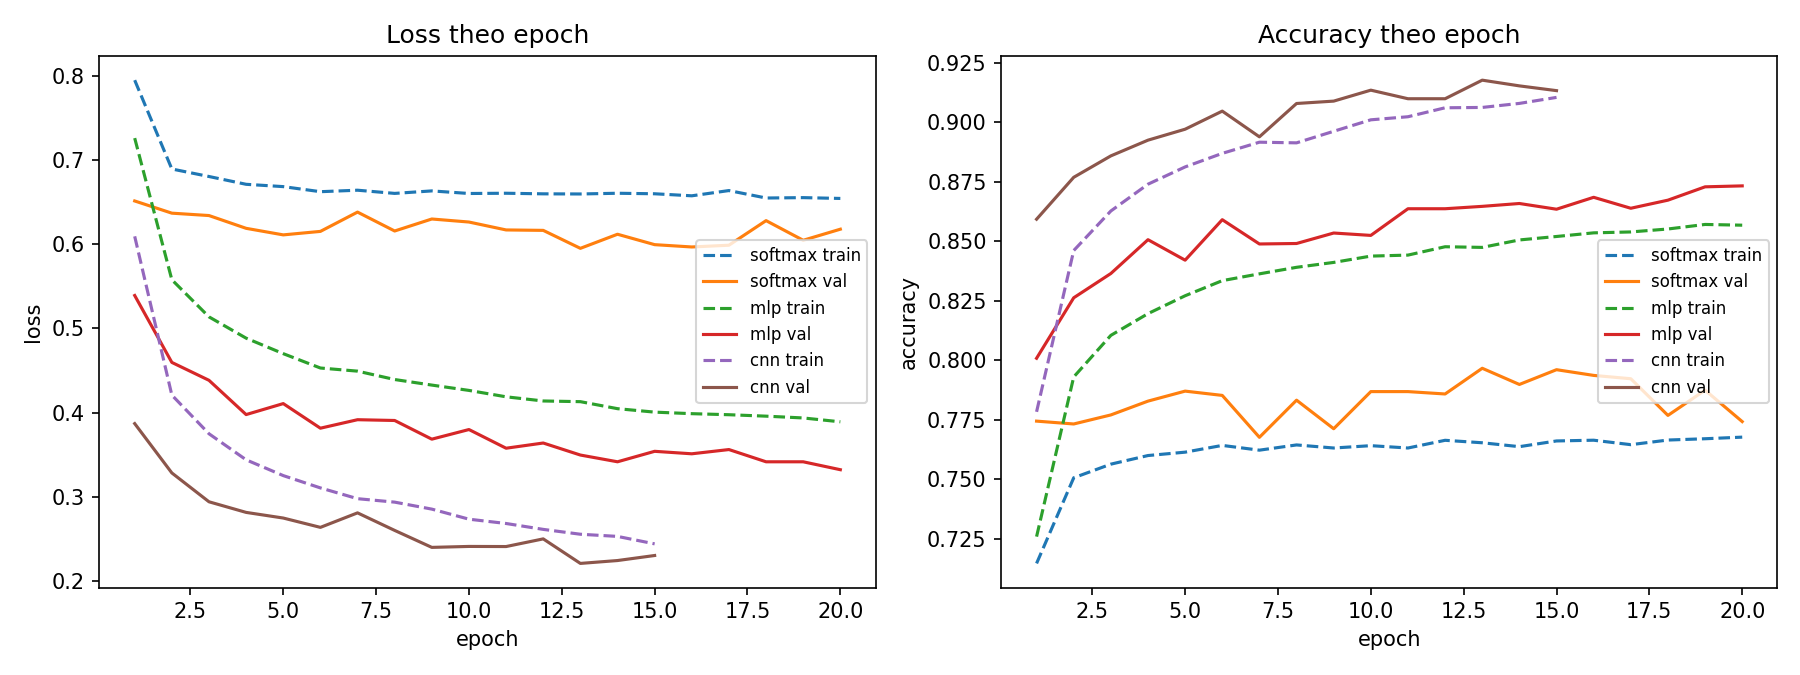
\includegraphics[width=\linewidth]{loss_accuracy_curves.png}
\caption{Đường cong loss và accuracy theo epoch của ba mô hình (nét đứt:
train, nét liền: validation)}
\label{fig:curves}
\end{figure}

Trên Hình~\ref{fig:curves}, ở cả MLP và CNN, accuracy trên tập train trong lúc
huấn luyện lại thấp hơn một chút so với validation, mặc dù thông thường train
accuracy phải cao hơn nếu mô hình overfit. Nguyên nhân là
Dropout chỉ được bật khi mô hình ở chế độ train: trong lúc tính train
accuracy, một phần neuron bị tắt ngẫu nhiên nên dự đoán khó hơn, trong khi lúc
đánh giá validation, Dropout tắt hoàn toàn nên mô hình dùng toàn bộ năng lực
đã học được. Đây không phải dấu hiệu underfit mà là hệ quả bình thường của
Dropout, và cũng cho thấy ở mức epoch đã chạy, cả MLP và CNN chưa có dấu hiệu
overfit rõ rệt (val loss vẫn đang giảm hoặc đi ngang chứ chưa tăng trở lại).
Riêng softmax, do capacity rất thấp, loss và accuracy trên cả train lẫn
validation bão hòa sớm và dao động nhẹ quanh một mức cố định suốt 20 epoch,
đặc trưng của underfitting hơn là overfitting.

\subsection{Phân tích lỗi}

\begin{figure}[H]
\centering
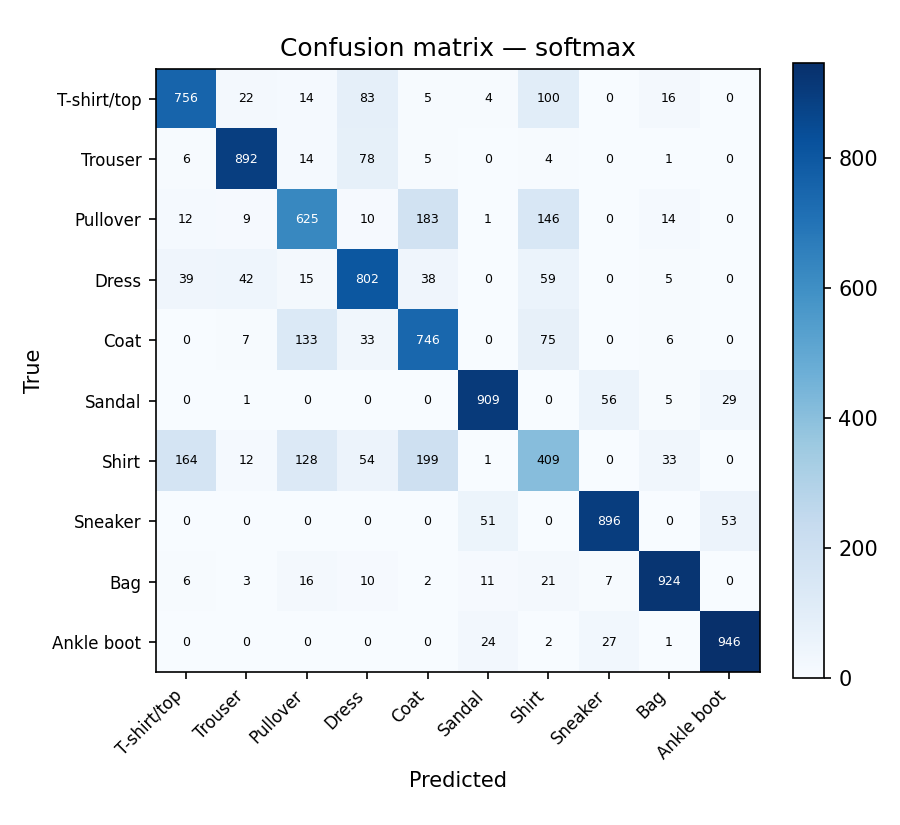
\includegraphics[width=0.75\linewidth]{confusion_matrix_softmax.png}
\caption{Confusion matrix của softmax trên tập test}
\end{figure}

\begin{figure}[H]
\centering
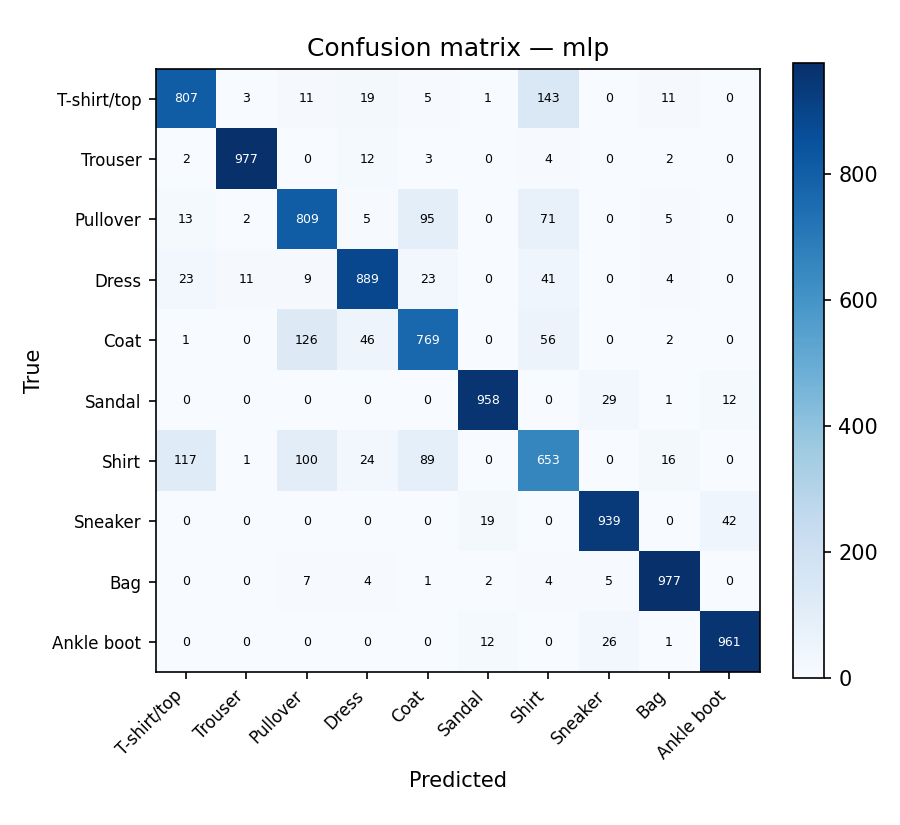
\includegraphics[width=0.75\linewidth]{confusion_matrix_mlp.png}
\caption{Confusion matrix của MLP trên tập test}
\end{figure}

\begin{figure}[H]
\centering
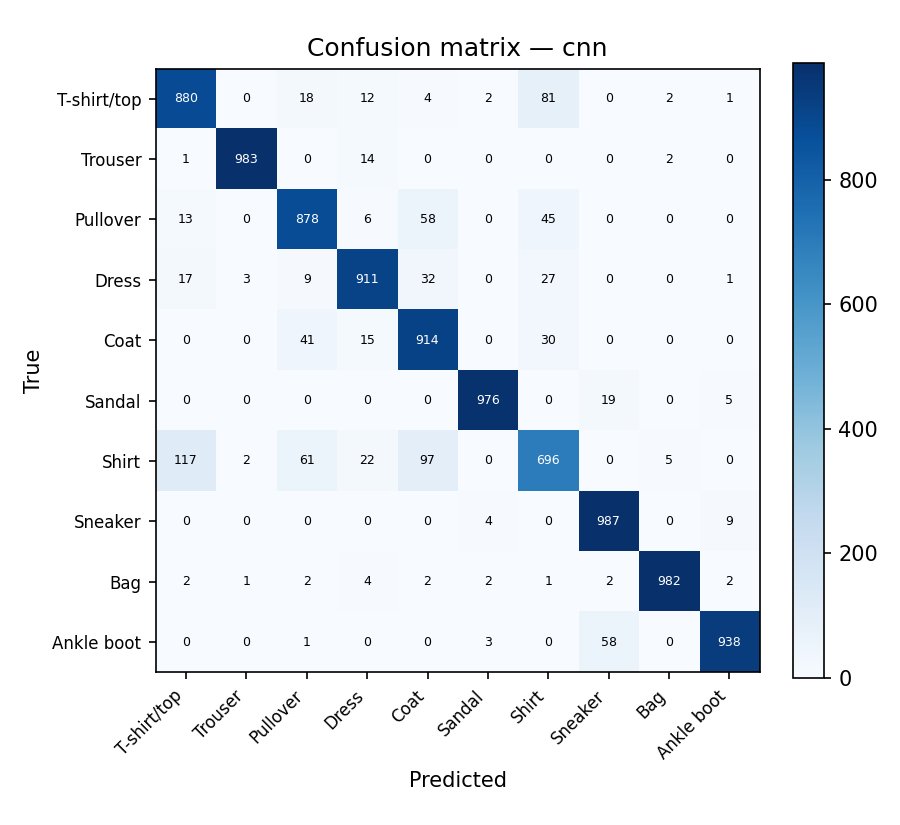
\includegraphics[width=0.75\linewidth]{confusion_matrix_cnn.png}
\caption{Confusion matrix của CNN trên tập test}
\label{fig:cm-cnn}
\end{figure}

Cả ba mô hình đều mắc lỗi tập trung ở cùng một cụm bốn lớp trang phục phần
thân trên: T-shirt/top, Pullover, Coat và Shirt. Đây là các lớp có hình dạng
tổng thể giống nhau (đều là áo nhìn thẳng, không tay hoặc có tay), khác nhau
chủ yếu ở chi tiết nhỏ như độ dày vải hay cổ áo, vốn khó phân biệt ở ảnh xám
$28\times28$. Lớp khó nhất với cả ba mô hình là \textbf{Shirt}:

\begin{itemize}
\item Softmax chỉ nhận đúng 409/1.000 ảnh Shirt (40,9\%), phần lớn bị nhầm
thành Coat (199 ảnh), Pullover (128 ảnh) và T-shirt/top (164 ảnh).
\item MLP nhận đúng 653/1.000 ảnh Shirt (65,3\%), lỗi giảm nhiều nhưng vẫn
nhầm sang T-shirt/top (117 ảnh), Pullover (100 ảnh) và Coat (89 ảnh).
\item CNN nhận đúng 696/1.000 ảnh Shirt (69,6\%), vẫn là lớp yếu nhất của
CNN nhưng đã tốt hơn MLP, lỗi còn lại chủ yếu vẫn rơi vào đúng ba lớp
T-shirt/top, Pullover, Coat.
\end{itemize}

Chiều ngược lại cũng xảy ra: T-shirt/top hay bị cả ba mô hình dự đoán nhầm
thành Shirt (100 ảnh ở softmax, 143 ảnh ở MLP, 81 ảnh ở CNN), và Pullover hay
bị nhầm thành Coat. Điều này cho thấy ranh giới quyết định giữa bốn lớp áo
phần thân trên là khó nhất trong toàn bộ bài toán, và việc tăng capacity hay
thêm convolution giúp thu hẹp vùng nhầm lẫn này chứ không loại bỏ hoàn toàn
được nó. Ngược lại, các lớp có hình dạng đặc trưng rõ (Trouser, Bag, Sandal,
Sneaker, Ankle boot) đều được cả ba mô hình nhận đúng trên 90\%, kể cả với
softmax tuyến tính đơn giản nhất.

\begin{figure}[H]
\centering
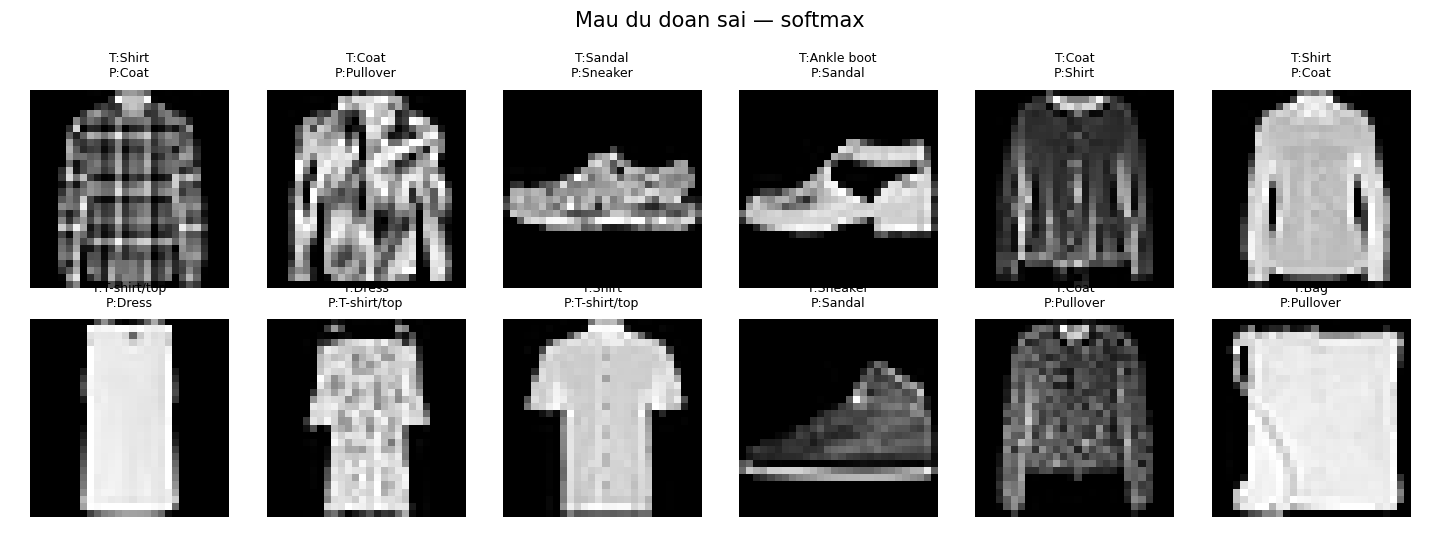
\includegraphics[width=\linewidth]{misclassified_softmax.png}
\caption{Một số ảnh bị softmax dự đoán sai (T: nhãn thật, P: nhãn dự đoán)}
\end{figure}

\begin{figure}[H]
\centering
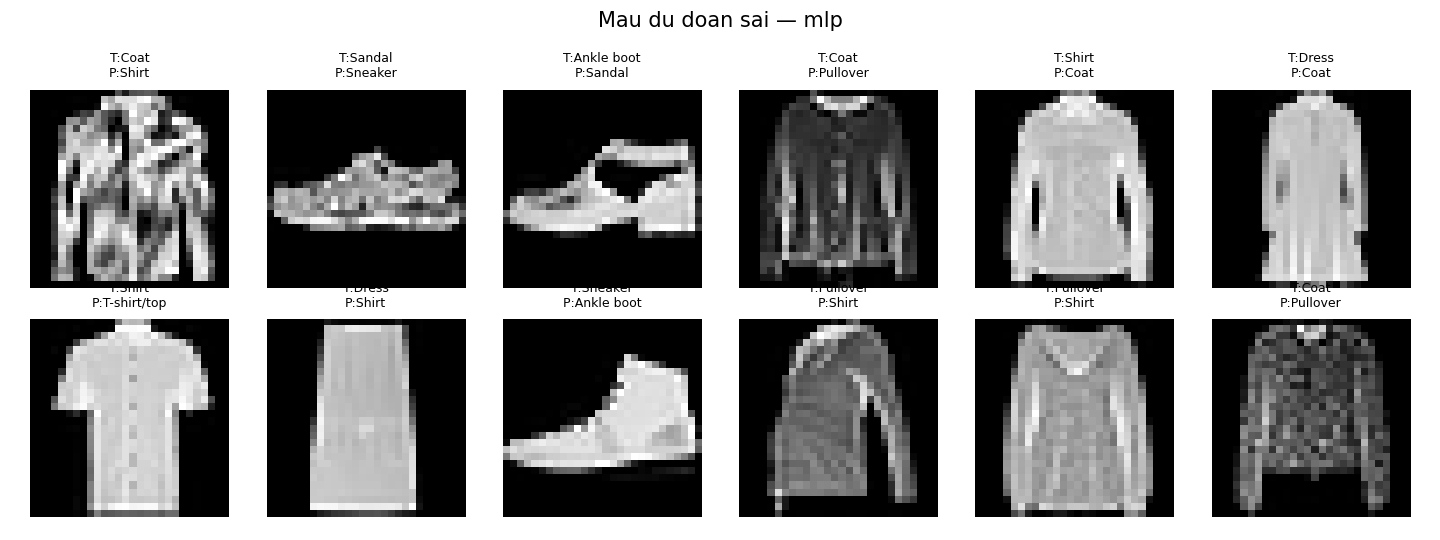
\includegraphics[width=\linewidth]{misclassified_mlp.png}
\caption{Một số ảnh bị MLP dự đoán sai}
\end{figure}

\begin{figure}[H]
\centering
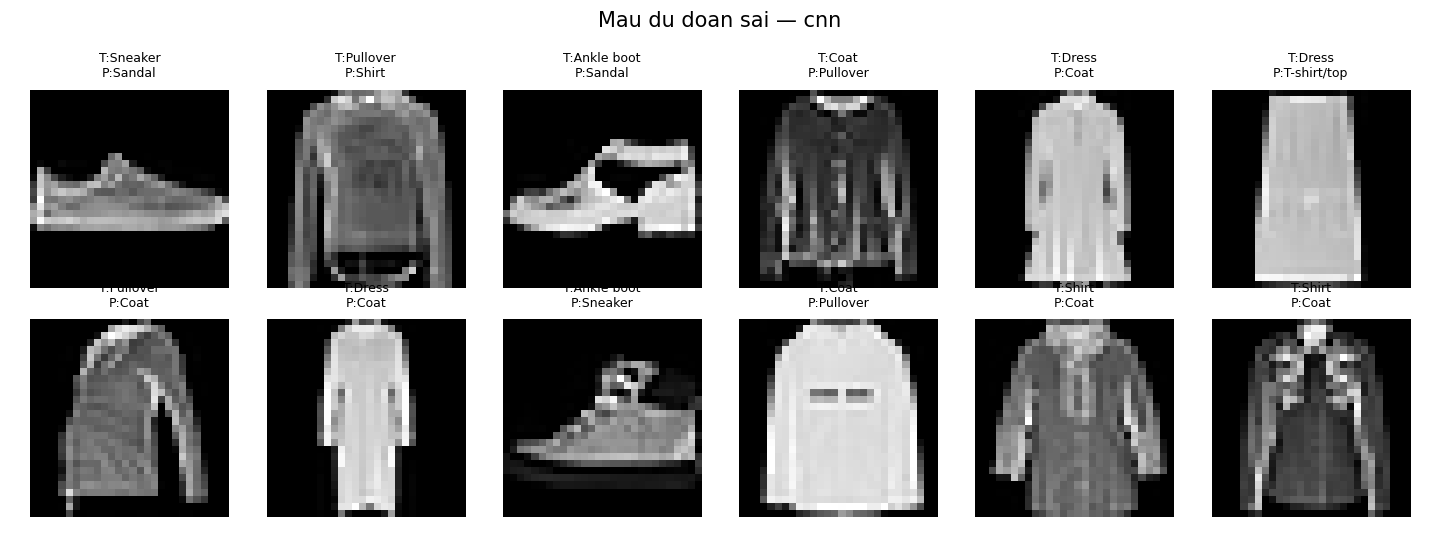
\includegraphics[width=\linewidth]{misclassified_cnn.png}
\caption{Một số ảnh bị CNN dự đoán sai}
\label{fig:misclassified-cnn}
\end{figure}

Quan sát trực tiếp các ảnh dự đoán sai ở Hình~\ref{fig:misclassified-cnn} cho
thấy phần lớn lỗi của CNN xảy ra ở những ảnh mà ngay cả người nhìn cũng khó
phân biệt dứt khoát, ví dụ một chiếc áo khoác mỏng bị gán nhãn Coat nhưng mô
hình dự đoán Pullover, hoặc một chiếc váy (Dress) ống rộng bị dự đoán thành
Coat. Đây là giới hạn vốn có của dữ liệu (ambiguity giữa các lớp) hơn là lỗi
của mô hình.

\subsection{Nhận xét}

Kết quả thực nghiệm cho thấy rõ sự đánh đổi giữa độ phức tạp kiến trúc và khả
năng phân loại: softmax tuyến tính đơn giản, huấn luyện ổn định nhưng capacity
quá thấp nên underfit, không tách được các lớp có ranh giới phi tuyến phức
tạp. MLP tăng capacity giúp accuracy tăng đáng kể, nhưng vẫn coi ảnh như một
vector phẳng, mất hoàn toàn thông tin cấu trúc không gian hai chiều của ảnh.
CNN đạt accuracy cao nhất với số tham số thấp hơn MLP ở các tầng trích đặc
trưng (nhờ weight sharing của convolution) và hội tụ nhanh hơn, vì kiến trúc
của nó phù hợp tự nhiên với dữ liệu ảnh. Cả ba mô hình đều gặp khó khăn giống
nhau ở cùng một cụm lớp trang phục phần thân trên, cho thấy giới hạn này đến
từ chính dữ liệu chứ không phải từ một kiến trúc cụ thể nào.

\clearpage
\section{E2: Transformer, MSA và tokenization}

Phần này sẽ được bổ sung trong lần cập nhật tiếp theo của báo cáo, cùng hạn
nộp với E1 (02/11/2026).

\clearpage
\section{E3: LSTM và GRU trên chuỗi ảnh}

Phần này sẽ được bổ sung trong lần cập nhật tiếp theo của báo cáo, đúng hạn
nộp của E3 (09/11/2026).

\end{document}
